\section{Methods}

\subsection{Overview of Methods}
Our plan of attack for this task was to try a few different types of methods and see which worked the best. In our proposal, we proposed the following:
\begin{itemize}
	\item Probabilistic models like Naive Bayes.
	\item Decision forests (Random Forest Classifiers)
\end{itemize}

However, we tried these approaches, and found that they performed very poorly on high dimensional, structured data like images. The assumptions on feature distributions in probabilistic models like Gaussian Naive Bayes do not hold at all here, and are therefore inappropriate. Models like RandomForest required extensive feature extraction, and did not give us correspondingly better results. Here we have shown a few methods that we thought were worth discussing. Our general pipeline consisted of 3 interconnected stages. The parts within a stage were options among many.
 
\begin{enumerate}
	\item \textbf{Stage 1 : Preprocessing}
	\begin{itemize}
		\item Data Preprocessing
		\begin{itemize}
			\item Resizing
			\item Grayscaling
			\item Scale Normalization
		\end{itemize}
		\item Data Augmentation: This consisted of primarily adding images to our dataset.
		\begin{itemize}
			\item Randomly Flipped/Rotated/Cropped and Resized copies
			\item Correcting class imbalances by oversampling under-represented classes (a lot of labeled whales had very few examples)
		\end{itemize}
		\item Keypoint detection and Matching
	\end{itemize}
	\item \textbf{Stage 2: Training}
	\begin{itemize}
		\item K-Nearest Neighbors
		\item Pretrained ImageNet models (ResNet18, ResNet152 ...)
		\item Bounding Boxes and ResNet50
	\end{itemize}
	\item \textbf{Stage 3: Post-processing and Testing}
	\begin{itemize}
		\item Labeling unidentified whales and adding top 5 predictions
	\end{itemize}
\end{enumerate}

We'll describe each of the three methods we tried to implement and discuss their merits and shortcomings.

\subsection{Keypoint Extraction, Matching and Classification}

One of the first and most naive implementations we tried was identifying keypoints in the training images and trying to match them to keypoints in test images with a brute-force matcher using OpenCV. Of course, the largest barrier to this method was the high resolution of most of the images. We downsampled the images and resized them to a uniform size before commencing with this method. 

\subsubsection{Keypoint Extraction}

We tried two main feature extraction methods namely, SIFT \cite{lowe2004distinctive} and ORB \cite{rublee2011orb}. Thankfully, there exists at least one version of opencv that provides functions for both detection and descriptor computation methods. Keypoints on whale tails are difficult to identify. In \cite{weideman2017integral}, Weideman et al. identified whales mainly by the contour of the edges of their tail flukes. Figure \ref{fig:whalekp} shows examples of whales with SIFT key points on the left and ORB keypoints on the right.

\begin{figure}[ht]
	\centering
	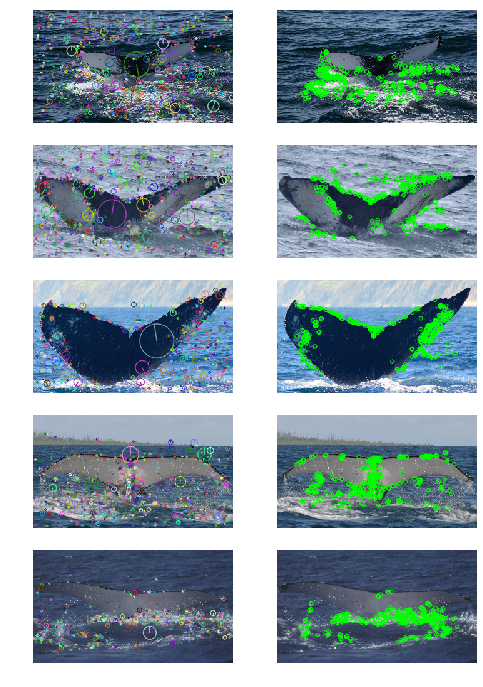
\includegraphics[width=.5\linewidth]{images/kp_side_by_side.png}
	\caption{\label{fig:whalekp}Left: SIFT keypoints. Right: ORB keypoints. Keypoints from the two methods drawn on some example whales}
\end{figure}
\begin{figure}[h]
	\centering
	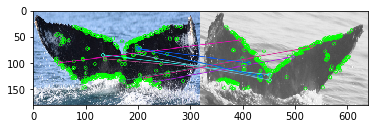
\includegraphics[width=.8\linewidth]{images/orb_matches.png}
	\caption{\label{fig:orbmatch}Matches between ORB keypoints between two tail flukes}
\end{figure}

\textit{A note on ORB vs SIFT descriptors:} We found, as seen above, that ORB was far more robust to the background noise due to the ocean than SIFT. ORB is also much faster, which for as many training/testing combinations we had, added up. For these reasons we decided to use ORB keypoints and descriptors for our naive implementation. 

\subsubsection{Keypoint Matching}

We used a brute force matcher using \textit{Hamming} distance as is normally done with ORB descriptors to calculate matches. Figure \ref{fig:orbmatch} shows an example match. This is how we were able to match keypoints between two images, but in order to score the matches, we had to compare them across all pairs of testing and training images. How do we score a pair of images? We decided to go with average match distance, since this was invariant to number of matches.

\subsubsection{Classification}

We decided to go with a K-Nearest Neighbor approach, as a first pass. In this approach, we took the average match distance matrix we had across all training and test pairs, and labeled each test image with the mode of the top K closest training images. Due to the low number of representatives for many classes it didn't make sense to have K$<$1, so we just took the label of the closest training image. Our results are in the Results section.

\subsection{Transfer learning using pretrained ResNet}

One of our main avenues of attack in trying to perform the classification task was to use transfer learning using a proven pretrained model. For this, we tried various versions of ResNet\textsuperscript{\cite{he2016deep}} - ResNet18, ResNet50, Resnet152 with various layers in each of the models frozen.

\subsubsection{Data Preprocessing and augmentation}

The first challenge in processing the images was that they were all of different sizes, and some were colored and some were grayscale. As part of preprocessing, we reduced all of them to a fixed size (for example 224x224 pixels) when loading them into memory. This was necessary since otherwise the images didn't fit in memory, which made the training process go really slow. We tried learning models with both grayscale as well as colored images, and we discovered that ResNet already works with colored images; and performance with colored images being better, we converted the single-channel grayscale images to ``colored'' ones by copying the grayscale channel to two more channels to imitate RGB.

The next major challenge was that the frequency of occurrences of whales (number of classes) in the trainining dataset was highly imbalanced as discussed in section \ref{subs:datachallenges}. To tackle this, we oversampled the underrepresented classes by adding copies of images to the training set to bring the frequency of all classes (whales) to 5 whales.

\subsubsection{Models}

We tried primarily to transfer learn using ResNet18 and Resnet152, and various configurations of frozen layers, learning rates, and preprocessing (without and with data augmentation). More information in the Results and Discussion sections.

\subsection{Bounding Boxes and ResNet50}

Our main method of noise reduction in the dataset (background ocean, small whale flukes) was to draw and crop to bounding boxes drawn around the whale in the image. Like many people in the original competition, our work was inspired and largely based on the initial work of the winner of the first Humpback Whale challenge, Martin Piotte \textsuperscript{\cite{martin}}, who trained a convolutional network model to estimate bounding boxes on the dataset.\\

Our architecture is loosely based on an adaptation of that network where we add 4 layers after a backbone of ResNet50. Table \ref{tab:bbres} shows a summary of the architecture we used. 

\begin{table}[h!]
	\centering
	\begin{tabular}{|c|}\hline
		\textbf{Layer}\\ \hline
		ResNet50 \\\hline
		BatchNorm1d \\ \hline
		Dropout \\ \hline
		Linear \\ \hline
		LogSoftMax \\ \hline
	\end{tabular}
	\caption{\label{tab:bbres} Bounding Box Model Architecture}
\end{table}

In addition to bounding boxes, we tried to further make the data more uniform by using a reference image in the training dataset for image alignment. Such a technique is used in facial detection and recognition. We computed descriptors and matched keypoints to compute a homography for each training image with this reference image. 